\documentclass[10pt,a4paper]{article}

\usepackage[margin=0.68in,top=0.68in,bottom=0.68in]{geometry}
\usepackage[T1]{fontenc}
\usepackage[utf8]{inputenc}
\usepackage{lmodern}
\usepackage{graphicx}
\usepackage{amsmath}
\usepackage{color}
\usepackage{colortbl}
\usepackage{tabularx}
\usepackage{array}
\usepackage{fancyhdr}
\usepackage[hidelinks]{hyperref}

\definecolor{navy}{RGB}{24,56,104}
\definecolor{slate}{RGB}{71,85,105}
\definecolor{rowtint}{RGB}{241,245,249}
\definecolor{headtint}{RGB}{226,232,240}

\setlength{\parindent}{0pt}
\setlength{\parskip}{3.5pt}
\setlength{\textfloatsep}{8pt plus 2pt minus 2pt}
\setlength{\intextsep}{7pt plus 2pt minus 2pt}
\setlength{\abovecaptionskip}{4pt}
\setlength{\belowcaptionskip}{2pt}
\renewcommand{\topfraction}{0.85}
\renewcommand{\bottomfraction}{0.85}
\renewcommand{\textfraction}{0.10}
\renewcommand{\floatpagefraction}{0.85}
\emergencystretch=2em

\pagestyle{fancy}
\fancyhf{}
\lhead{\small\color{slate}HUST --- IT4931 Individual Course Report}
\rhead{\small\color{slate}Nguy\~{\^e}n Danh Th\'ai --- MSSV: 202400072}
\cfoot{\small\thepage}
\renewcommand{\headrulewidth}{0.4pt}

\makeatletter
\renewcommand{\section}{\@startsection{section}{1}{\z@}{-9pt plus -2pt minus -2pt}{4pt plus 1pt}{\large\bfseries\color{navy}}}
\renewcommand{\subsection}{\@startsection{subsection}{2}{\z@}{-6pt plus -1pt minus -1pt}{2.5pt plus 1pt}{\normalsize\bfseries\color{navy}}}
\makeatother

\newcolumntype{L}{>{\raggedright\arraybackslash}X}

\begin{document}

\begin{center}
    {\small\scshape Hanoi University of Science and Technology (HUST) --- School of ICT}\\[2pt]
    {\Large\bfseries\color{navy} Design and Empirical Evaluation of a Lambda Data Pipeline}\\[3pt]
    {\normalsize Course Report: IT4931 --- Batch-Only (Arch A) vs.\ Lambda Architecture (Arch B)}\\[3pt]
    {\small Student: \textbf{Nguy\~{\^e}n Danh Th\'ai} \quad|\quad MSSV: \textbf{202400072} \quad|\quad GitHub: \texttt{github.com/Choe222/Lambda-Architecture}}
\end{center}
\vspace{-4pt}
\hrule
\vspace{5pt}

\noindent\textbf{Abstract.}
In this individual project, I implemented and empirically evaluated two event-aggregation pipelines over real NYC Yellow Taxi trip records using Apache Kafka, PySpark (Batch and Structured Streaming), and PostgreSQL: a periodic \textbf{Batch-only} baseline (Arch~A, 30\,s cycle) and a \textbf{Lambda} pipeline (Arch~B) combining an immutable batch layer with an idempotent speed layer via a contiguous sequence watermark $H$. Across 16 independent benchmark runs spanning five experiment groups (E1--E5), Arch~B achieved \textbf{100\% exact reconciliation} against ground truth (\texttt{count\_diff = 0}, \texttt{sum\_diff\_cents = 0}) while cutting p95 end-to-end freshness by \textbf{28.6$\times$} at 20\,eps (50.14\,s $\rightarrow$ 1.76\,s) and \textbf{14.3$\times$} at 100\,eps (68.75\,s $\rightarrow$ 4.81\,s). Profiling exposed row-by-row PostgreSQL commits and Spark's default 200 shuffle partitions as the main bottlenecks; replacing them with batched \texttt{execute\_values} upserts and tuned parallelism in E4 reduced p95 freshness by \textbf{66.3\%} (to 1.62\,s, a \textbf{2.97$\times$} speedup) and halved batch runtime (22.20\,s $\rightarrow$ 10.73\,s) on unchanged hardware.

\section{Problem Statement and Dataset Preparation}
Analytic systems face a fundamental tension between \emph{low update latency} and \emph{exact recomputability}. Batch pipelines recompute clean snapshots over immutable raw logs but delay visibility until the next batch cycle completes. The Lambda architecture preserves an authoritative batch layer while introducing a parallel streaming speed layer to serve recent events immediately, provided both layers merge at the serving tier without double counting or temporary drops.

\textbf{Real Public Dataset.}
Using \texttt{prepare\_data.py}, we ingested the January 2024 NYC TLC Yellow Taxi Trip dataset (\texttt{yellow\_tripdata\_2024-01.parquet}, SHA-256 \texttt{c4d59da7...b2030510}). Out of \textbf{2,964,624} raw rows, \textbf{102,998} invalid records were filtered out (null timestamps/zones/amounts, \texttt{total\_amount} $\notin (0, 1000]$, trip distance $\le 0$, or pickup zone $\notin [1, 263]$), leaving \textbf{2,861,626} valid records. From these, \textbf{25,000} rows were deterministically sampled (\texttt{seed=42}), sorted chronologically, and stored in \texttt{data/cleaned\_events.parquet} alongside \texttt{data/data\_manifest.json} and a 1,000-row sample CSV.

\begin{table}[htbp]
\centering
\footnotesize
\setlength{\tabcolsep}{4pt}
\begin{tabularx}{\textwidth}{|l|X|}
\hline
\rowcolor{headtint} \textbf{Field} & \textbf{Specification and Role in Pipeline} \\
\hline
\texttt{event\_id} & Deterministic 24-char SHA-256 prefix of \texttt{(event\_time, category, amount\_cents, seq)}; primary deduplication key. \\
\rowcolor{rowtint} \texttt{seq} & Monotonically increasing integer $1, 2, 3, \dots$ assigned by a single producer on Kafka partition~0. \\
\texttt{event\_time} & Original trip pickup timestamp from the NYC TLC dataset (ISO-8601 UTC string); preserved as business metadata. \\
\rowcolor{rowtint} \texttt{produced\_at} & Live wall-clock UTC timestamp recorded at emission; baseline $t_0$ for end-to-end freshness measurement. \\
\texttt{category} & Grouping key mapped across 10 balanced buckets: \texttt{"ZONE\_" + (PULocationID \% 10)} (\texttt{ZONE\_0}--\texttt{ZONE\_9}). \\
\rowcolor{rowtint} \texttt{amount\_cents} & Integer monetary value $\text{round}(\text{total\_amount} \times 100)$ to eliminate floating-point rounding drift in \texttt{SUM}. \\
\hline
\end{tabularx}
\caption{Normalized event schema (\texttt{prepare\_data.py} and \texttt{producer.py}). Replay pace uses configurable constant/burst rates.}
\end{table}

\section{Lambda Architecture and Correctness Guarantees}
Figure~\ref{fig:arch} illustrates the complete end-to-end system. Both Arch~A and Arch~B share the exact same Kafka ingestion path and immutable Parquet archiving path so storage costs are accounted for identically.

\begin{figure}[htbp]
\centering
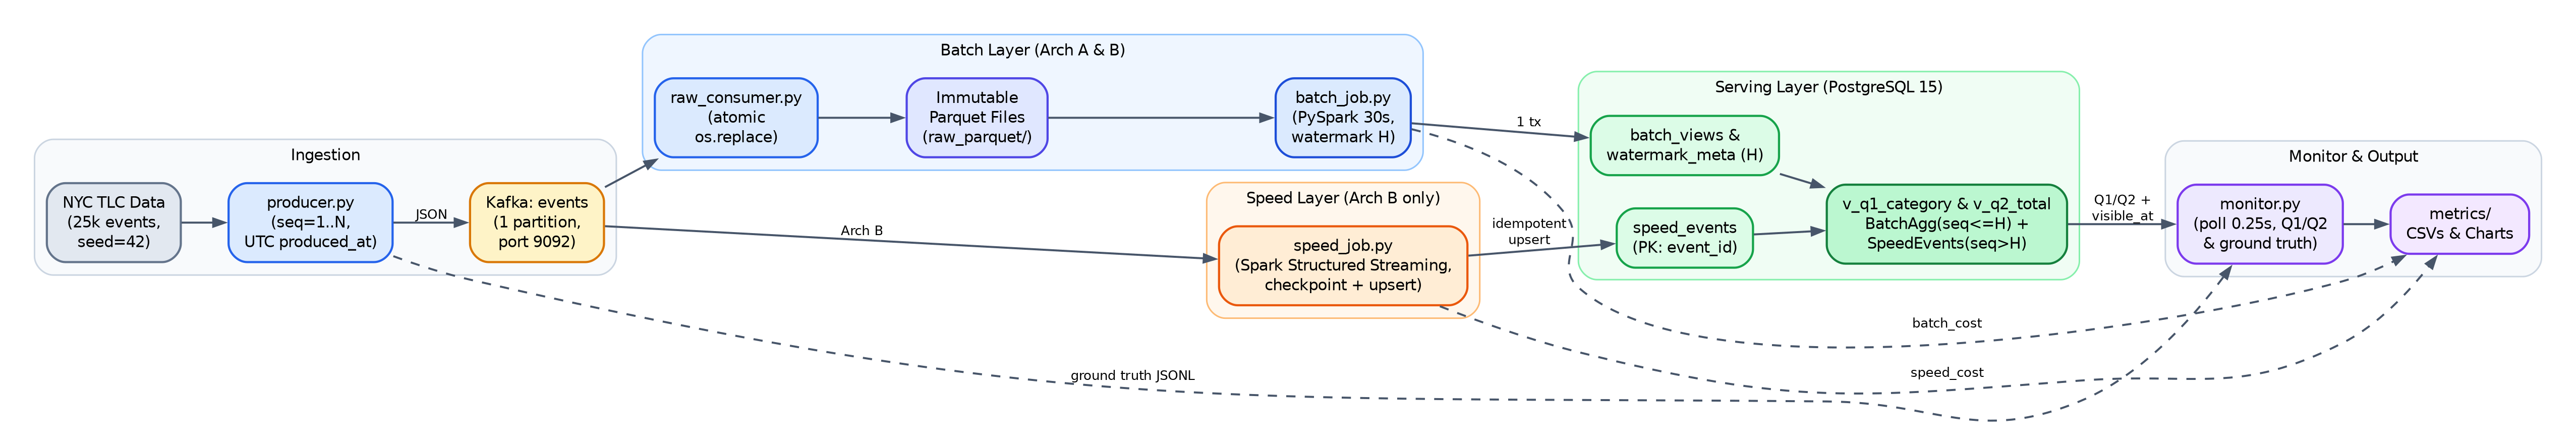
\includegraphics[width=\textwidth]{../docs/architecture.png}
\caption{End-to-end Lambda pipeline architecture. Arch~A omits \texttt{speed\_job.py}; Arch~B runs both layers concurrently.}
\label{fig:arch}
\end{figure}

\textbf{Ingestion \& Atomic Raw Storage.}
\texttt{producer.py} replays normalized events into a 1-partition Kafka topic (\texttt{events}) while logging every emitted record to \texttt{logs/produced\_ground\_truth.jsonl}. \texttt{raw\_consumer.py} consumes messages with manual offset commits (\texttt{enable\_auto\_commit=False}), buffers up to 500 events or 3.0\,s, writes each Parquet chunk to \texttt{raw\_tmp/}, and atomically promotes it to \texttt{raw\_parquet/part\_<min>\_<max>\_<ts>.parquet} via \texttt{os.replace()}. Batch readers therefore never observe partial files.

\textbf{Contiguous Watermark $H$ \& Transactional Merge.}
Every 30\,s (and on clean shutdown), \texttt{batch\_job.py} inspects Parquet filename intervals $[\text{min\_seq}, \text{max\_seq}]$ and computes the highest contiguous prefix $H$ with zero sequence gaps starting from $1$. It aggregates \texttt{COUNT(*)} and \texttt{SUM(amount\_cents)} for $\text{seq} \le H$, then updates \texttt{batch\_views}, advances \texttt{watermark\_meta.h\_seq = H}, and records newly covered events in \texttt{batch\_seen\_events} inside a \textbf{single PostgreSQL transaction}. Meanwhile, in Arch~B, \texttt{speed\_job.py} maintains a Structured Streaming checkpoint in \texttt{checkpoints/speed/} and inserts events into \texttt{speed\_events} with \texttt{ON CONFLICT (event\_id) DO NOTHING}. Serving views \texttt{v\_q1\_category} and \texttt{v\_q2\_total} compute:
\[
    \text{ServingResult} \;=\; \text{BatchAgg}(\text{seq} \le H) \;+\; \text{SpeedEvents}(\text{seq} > H)
\]
Because \texttt{batch\_views} and \texttt{h\_seq} commit atomically under PostgreSQL MVCC snapshot isolation, concurrent Q1/Q2 queries never transiently double-count or omit boundary events when $H$ advances.

\section{Experimental Setup and Methodology}
All 16 experiments ran sequentially on a dedicated single host so Arch~A and Arch~B never competed for resources. Before every run, \texttt{run\_experiment.py} cleared \texttt{raw\_parquet/}, \texttt{raw\_tmp/}, \texttt{checkpoints/}, and \texttt{logs/}, verified deletion and recreation of Kafka topic \texttt{events}, and re-applied \texttt{sql/schema.sql}.

\begin{itemize}\setlength{\itemsep}{1pt}\setlength{\parskip}{0pt}
    \item \textbf{Host \& Runtime Versions:} Intel Core i5-10300H (4 cores / 8 threads @ 2.50\,GHz), 7.6\,GiB RAM (+ 3.8\,GiB swap), Arch Linux (kernel 7.2.9); Python 3.14.8, PySpark 4.3.0, OpenJDK 17.0.21, Apache Kafka 3.7.0, PostgreSQL 15-alpine, Docker 29.9.0.
    \item \textbf{Measurement Protocol:} 120\,s emission window; first 20\,s designated as warm-up (excluded from active metrics and freshness sampling); 0.25\,s polling interval with 81--82 uniformly timed samples per run (0 unseen). Freshness measures $\max(\text{visible\_at}, \text{produced\_at}) - \text{produced\_at}$ directly in PostgreSQL, not Spark job execution time.
\end{itemize}

\begin{table}[htbp]
\centering
\footnotesize
\setlength{\tabcolsep}{4pt}
\begin{tabularx}{\textwidth}{|l|c|l|c|c|X|}
\hline
\rowcolor{headtint} \textbf{Suite} & \textbf{Arch} & \textbf{Workload} & \textbf{Spark Res.} & \textbf{Runs} & \textbf{Evaluation Objective} \\
\hline
E1 (Low Load) & A, B & 20\,eps constant $\times$ 120\,s & 2c / 2\,GB & 2 + 2 & Freshness benefit vs.\ baseline resource overhead. \\
\rowcolor{rowtint} E2 (High Load) & A, B & 100\,eps constant $\times$ 120\,s & 2c / 2\,GB & 2 + 2 & Sustained throughput, backlog growth, SQL cost. \\
E3 (Burst) & B & 20 $\rightarrow$ 150 $\rightarrow$ 20\,eps (40\,s phases) & 2c / 2\,GB & 2 & Overload accumulation and drain recovery speed. \\
\rowcolor{rowtint} E4 (Optimized) & B (\texttt{--opt}) & 100\,eps constant $\times$ 120\,s & 2c / 2\,GB & 2 & Controlled bottleneck fix on identical hardware. \\
E5 (Scale-up) & B & 100\,eps constant $\times$ 120\,s & 2c/2g vs 4c/4g & 2 + 2 & Observed vertical speedup $S$ and efficiency $E$. \\
\hline
\end{tabularx}
\caption{Benchmark experiment suite (16 runs total; sequential execution with full state reset between runs).}
\end{table}

\section{Benchmark Results: Baseline, High Load, and Burst (E1--E3)}
Table~\ref{tab:agg} summarizes the mean metrics across all 8 experiment groups (2 independent runs per group). Every single run reconciled with \textbf{zero event count or cent discrepancies} (\texttt{count\_diff = 0}, \texttt{sum\_diff\_cents = 0}).

\begin{table}[htbp]
\centering
\resizebox{\textwidth}{!}{%
\begin{tabular}{|l|l|r|r|r|r|r|r|r|r|r|r|c|}
\hline
\rowcolor{headtint}
\textbf{Group} & \textbf{Configuration} & \textbf{p50 (ms)} & \textbf{p95 (ms)} & \textbf{Tput (eps)} & \textbf{Avg Bk} & \textbf{Max Bk} & \textbf{CPU\%} & \textbf{RAM (MB)} & \textbf{Q1 p95} & \textbf{Batch (s)} & \textbf{Diff} & \textbf{OK} \\
\hline
\texttt{E1\_A} & A, 20\,eps, 2c/2g & 28,643.1 & 50,143.1 & 15.81 & 636.0 & 1,095 & 38.0 & 5,874.7 & 3.46 & 9.76 & 0 & Yes \\
\rowcolor{rowtint} \texttt{E1\_B} & B, 20\,eps, 2c/2g & 871.6 & 1,755.4 & 21.63 & 18.7 & 202 & 62.1 & 6,559.0 & 7.97 & 16.58 & 0 & Yes \\
\texttt{E2\_A} & A, 100\,eps, 2c/2g & 38,862.8 & 68,749.5 & 65.14 & 4,641.8 & 7,440 & 69.4 & 6,190.1 & 5.22 & 17.61 & 0 & Yes \\
\rowcolor{rowtint} \texttt{E2\_B} & B, 100\,eps, 2c/2g & 1,314.2 & 4,806.4 & 117.12 & 295.3 & 2,120 & 82.6 & 6,519.7 & 25.18 & 22.20 & 0 & Yes \\
\texttt{E3\_B} & B, burst, 2c/2g & 971.8 & 2,787.6 & 72.70 & 138.0 & 537 & 69.8 & 6,033.5 & 20.23 & 18.57 & 0 & Yes \\
\rowcolor{rowtint} \texttt{E4\_B\_opt} & B, 100\,eps, opt & 724.1 & 1,620.5 & 113.52 & 123.8 & 1,301 & 80.1 & 5,901.4 & 15.97 & 10.73 & 0 & Yes \\
\texttt{E5\_C1} & B, 100\,eps, 2c/2g & 1,018.5 & 1,575.3 & 100.88 & 102.7 & 211 & 67.7 & 6,080.5 & 15.07 & 15.45 & 0 & Yes \\
\rowcolor{rowtint} \texttt{E5\_C2} & B, 100\,eps, 4c/4g & 980.0 & 1,710.8 & 103.30 & 104.0 & 347 & 66.6 & 6,227.0 & 13.92 & 13.71 & 0 & Yes \\
\hline
\end{tabular}%
}
\caption{Aggregated benchmark results (mean over 2 runs per group; Diff = $\max(|\text{count\_diff}|, |\text{sum\_diff\_cents}|)$). Q1 p95 in ms.}
\label{tab:agg}
\end{table}

\textbf{Batch-Only vs.\ Lambda (E1 \& E2).}
As shown in Figure~\ref{fig:c12}\,(left), Batch-only (Arch~A) suffers tens of seconds of staleness governed by its 30\,s schedule plus Spark execution time: p95 freshness reaches \textbf{50.14\,s} at 20\,eps and \textbf{68.75\,s} at 100\,eps, with unserved backlog climbing to \textbf{7,440 events} between snapshots. Adding the speed layer reduces p95 freshness by \textbf{28.6$\times$} in E1 (to \textbf{1.76\,s}) and \textbf{14.3$\times$} in E2 (to \textbf{4.81\,s}), keeping active throughput tightly aligned with the input rate. However, this comes at measurable resource cost: running two concurrent Spark JVMs raises average CPU by \textbf{+24.1\,pp} in E1 (38.0\% $\rightarrow$ 62.1\%) and \textbf{+13.3\,pp} in E2 (69.4\% $\rightarrow$ 82.6\%), adds up to \textbf{684\,MB} of host RAM, and increases Q1 query p95 latency from 5.22\,ms to 25.18\,ms in E2 because PostgreSQL must aggregate unmerged \texttt{speed\_events} rows alongside \texttt{batch\_views}.

\textbf{Burst Overload \& Recovery (E3).}
Figure~\ref{fig:c12}\,(right) traces \texttt{E3\_B\_burst\_run1} across its 40\,s phases (20 $\rightarrow$ 150 $\rightarrow$ 20\,eps). During initial cold-start warmup ($t < 25$\,s), Spark Structured Streaming pulls Kafka metadata and compiles its first micro-batch, briefly building a 480-event backlog before catching up before $t=30$\,s. When traffic surges 7.5$\times$ to 150\,eps ($t=40$--$80$\,s), serial JDBC commits fall behind, creating sawtooth backlog peaks up to \textbf{537 events}. Once traffic drops back to 20\,eps at $t=80$\,s, the speed layer drains the backlog within \textbf{$\sim$3--4\,s}, maintains steady 20\,eps serving thereafter, and finishes all \textbf{7,596} events with zero loss or duplication.

\begin{figure}[htbp]
\centering
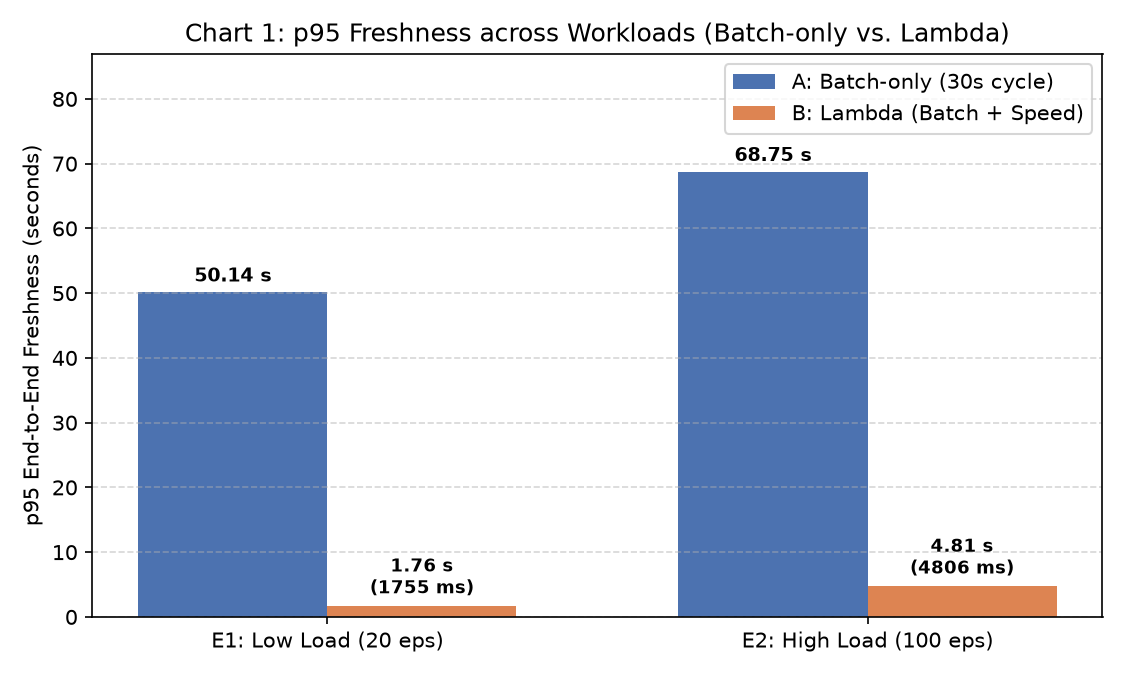
\includegraphics[width=0.495\textwidth]{../metrics/charts/chart1_freshness_comparison.png}\hfill
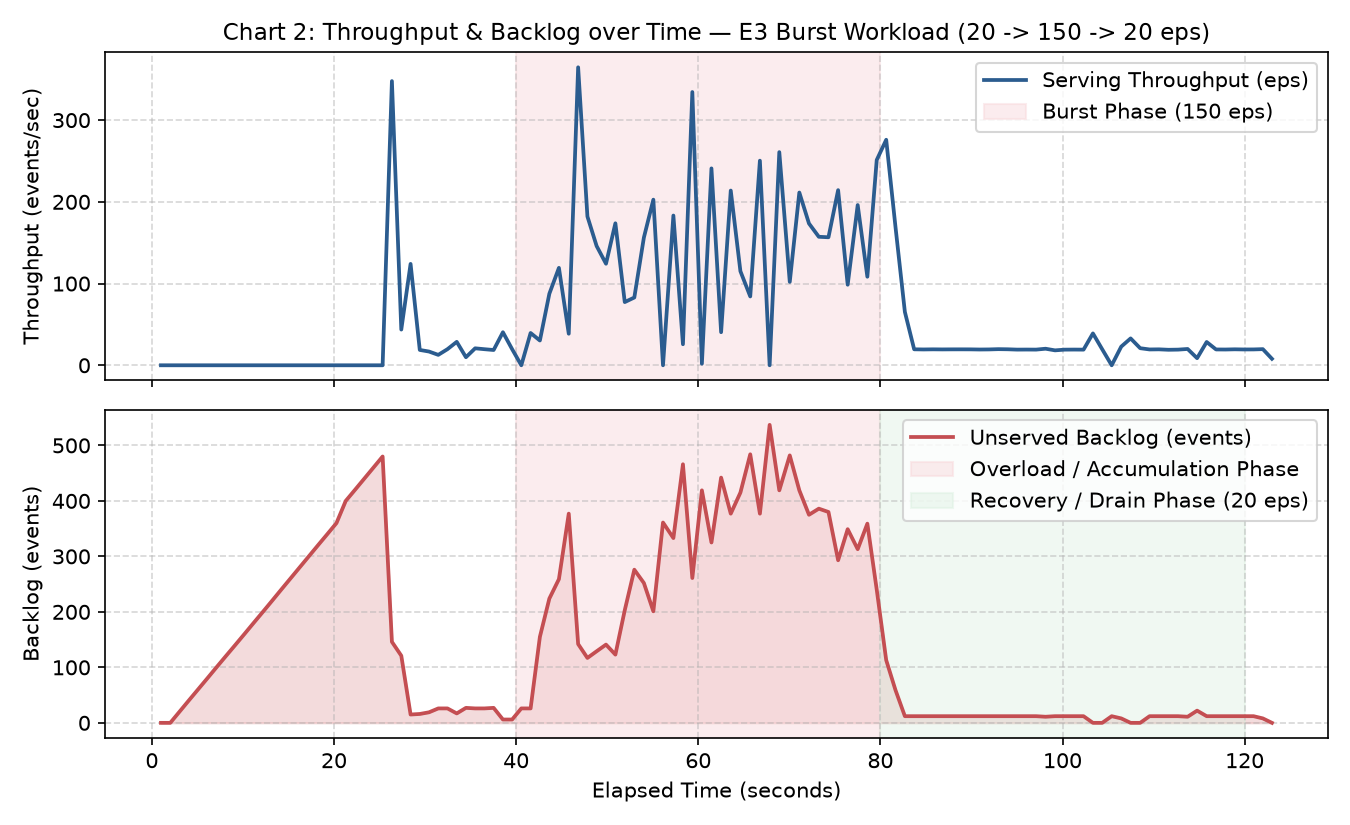
\includegraphics[width=0.495\textwidth]{../metrics/charts/chart2_throughput_backlog_timeseries.png}
\caption{Left: E1/E2 p95 freshness comparison (Chart~1). Right: E3 burst throughput and backlog recovery over time (Chart~2).}
\label{fig:c12}
\end{figure}

\section{Bottleneck Analysis and Verified Optimization (E4)}
\textbf{1. Bottleneck Evidence.}
In \texttt{E2\_B} (100\,eps, 2c/2g), \texttt{speed\_cost.csv} logged \textbf{168 micro-batches} averaging \textbf{142.9 records} with a mean PostgreSQL write time of \textbf{849.6\,ms} and p95 write time of \textbf{1,593.0\,ms}---exceeding the 1,000\,ms trigger interval and driving max backlog to \textbf{2,120 events} and p95 freshness to \textbf{4,806\,ms}. Concurrently, \texttt{batch\_job.py} averaged \textbf{22.20\,s} per run (peaking at \textbf{47.47\,s}), creating heavy CPU contention (82.6\% avg).

\textbf{2. Root-Cause Hypothesis.}
Two implementation inefficiencies compounded on the 2-core host: (a) \texttt{speed\_job.py} executed an individual \texttt{INSERT ... ON CONFLICT DO NOTHING} plus \texttt{conn.commit()} \emph{per event} ($\sim$143 separate WAL fsync round-trips per micro-batch), and (b) both Spark jobs retained the default \texttt{spark.sql.shuffle.partitions = 200}, scheduling 200 shuffle tasks for small 12,000-row datasets across 2 local threads.

\textbf{3. Before/After Optimization (\texttt{--opt}).}
Holding Spark hardware resources fixed at 2 cores / 2\,GB, Table~\ref{tab:opt} details the coordinated write and shuffle configuration change verified in E4.

\begin{table}[htbp]
\centering
\footnotesize
\setlength{\tabcolsep}{5pt}
\begin{tabularx}{\textwidth}{|l|L|L|}
\hline
\rowcolor{headtint} \textbf{Parameter / Path} & \textbf{E2 Baseline (\texttt{opt=False})} & \textbf{E4 Optimized (\texttt{--opt})} \\
\hline
PostgreSQL speed upsert & Per-row \texttt{cur.execute()} + \texttt{conn.commit()} & Single-tx \texttt{execute\_values(..., page\_size=1000)} \\
\rowcolor{rowtint} \texttt{spark.sql.shuffle.partitions} & \texttt{200} (excess task scheduling on 2 cores) & \texttt{4} (matched to \texttt{local[2]} parallelism) \\
Streaming trigger / batch cap & \texttt{1 second} trigger, \texttt{maxOffsets=500} & \texttt{200 milliseconds} trigger, \texttt{maxOffsets=5000} \\
\hline
\end{tabularx}
\caption{Controlled E4 optimization settings (\texttt{speed\_job.py} and \texttt{batch\_job.py}); CPU/RAM fixed at 2 cores / 2\,GB.}
\label{tab:opt}
\end{table}

\textbf{4. E2 vs.\ E4 Results.}
As shown in Figure~\ref{fig:c3}, E4 improved every latency, backlog, and resource metric simultaneously: p95 freshness fell \textbf{66.3\%} (4,806 $\rightarrow$ \textbf{1,621\,ms}, a \textbf{2.97$\times$} speedup), p50 freshness fell \textbf{44.9\%} (1,314 $\rightarrow$ \textbf{724\,ms}), speed write p95 fell \textbf{59.5\%} (1,593 $\rightarrow$ \textbf{645\,ms}), max backlog fell \textbf{38.7\%} (2,120 $\rightarrow$ \textbf{1,301 events}), and average batch job runtime fell \textbf{51.7\%} (22.20\,s $\rightarrow$ \textbf{10.73\,s}). Faster watermark progression also pruned \texttt{speed\_events} scans, cutting Q1 p95 query latency by \textbf{36.6\%} (25.18 $\rightarrow$ \textbf{15.97\,ms}) while lowering average CPU (82.6\% $\rightarrow$ \textbf{80.1\%}) and RAM (6,520 $\rightarrow$ \textbf{5,901\,MB}).

\textbf{5. Trade-offs \& Recommendation.}
The 200\,ms trigger generates 2.2$\times$ more micro-batch checkpoints (369 vs.\ 168), and \texttt{shuffle.partitions=4} must be scaled up if batch data grows to multi-gigabyte volumes. Because it yields nearly 3$\times$ better freshness and halves batch cost on identical hardware, \textbf{the E4 optimization should be adopted in production}.

\begin{figure}[!htbp]
\centering
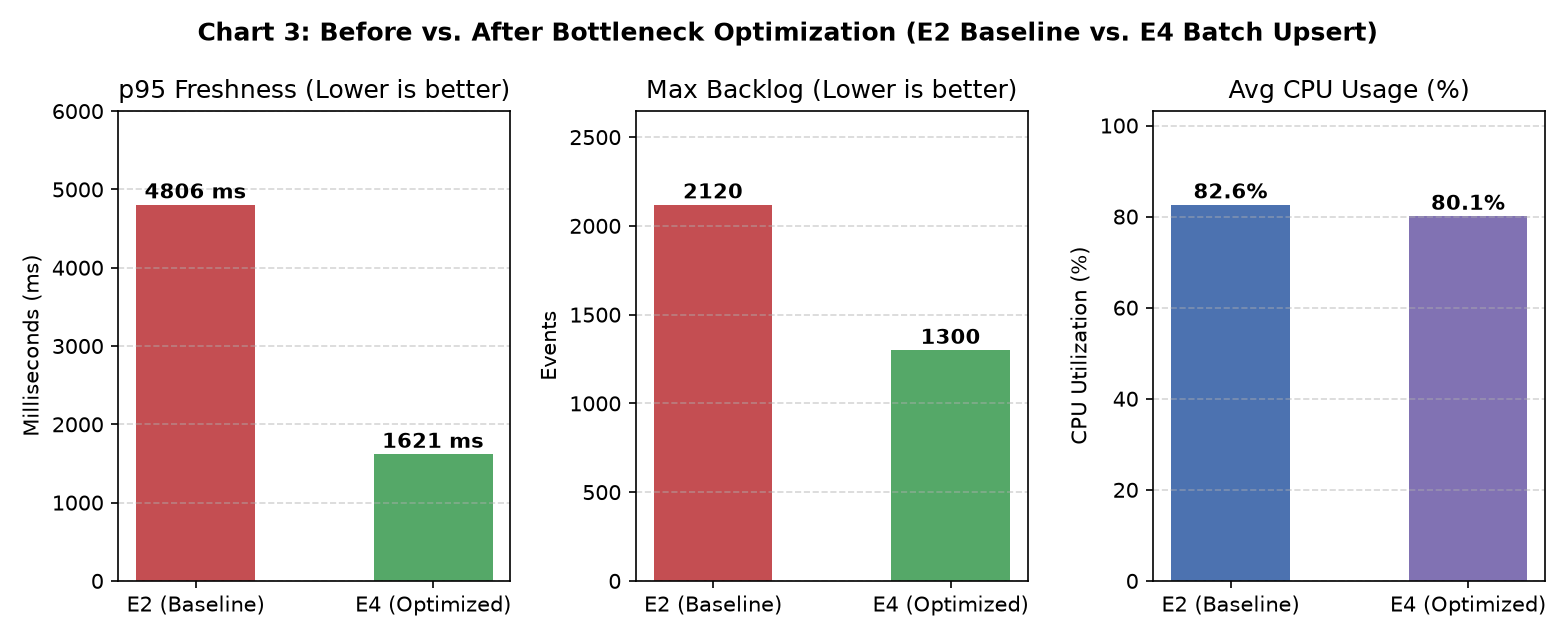
\includegraphics[width=0.68\textwidth]{../metrics/charts/chart3_e2_vs_e4_optimization.png}
\caption{Chart~3: Before vs.\ after bottleneck optimization on identical 2-core / 2\,GB hardware (E2 baseline vs.\ E4 batch upsert).}
\label{fig:c3}
\end{figure}

\section{Vertical Scalability Evaluation (E5)}
To assess vertical scaling without modifying application logic (baseline row-by-row mode), we ran workload E2 (100\,eps) under \textbf{C1} (2 cores / 2\,GB) and \textbf{C2} (4 cores / 4\,GB) in Figure~\ref{fig:c4}. Average serving throughput moved from \textbf{100.88\,eps} (C1) to \textbf{103.30\,eps} (C2), yielding an observed speedup $S = 103.30 / 100.88 = \mathbf{1.02\times}$ and observed scaling efficiency $E = (1.024 / 2) \times 100\% = \mathbf{51.2\%}$.

\begin{figure}[!htbp]
\centering
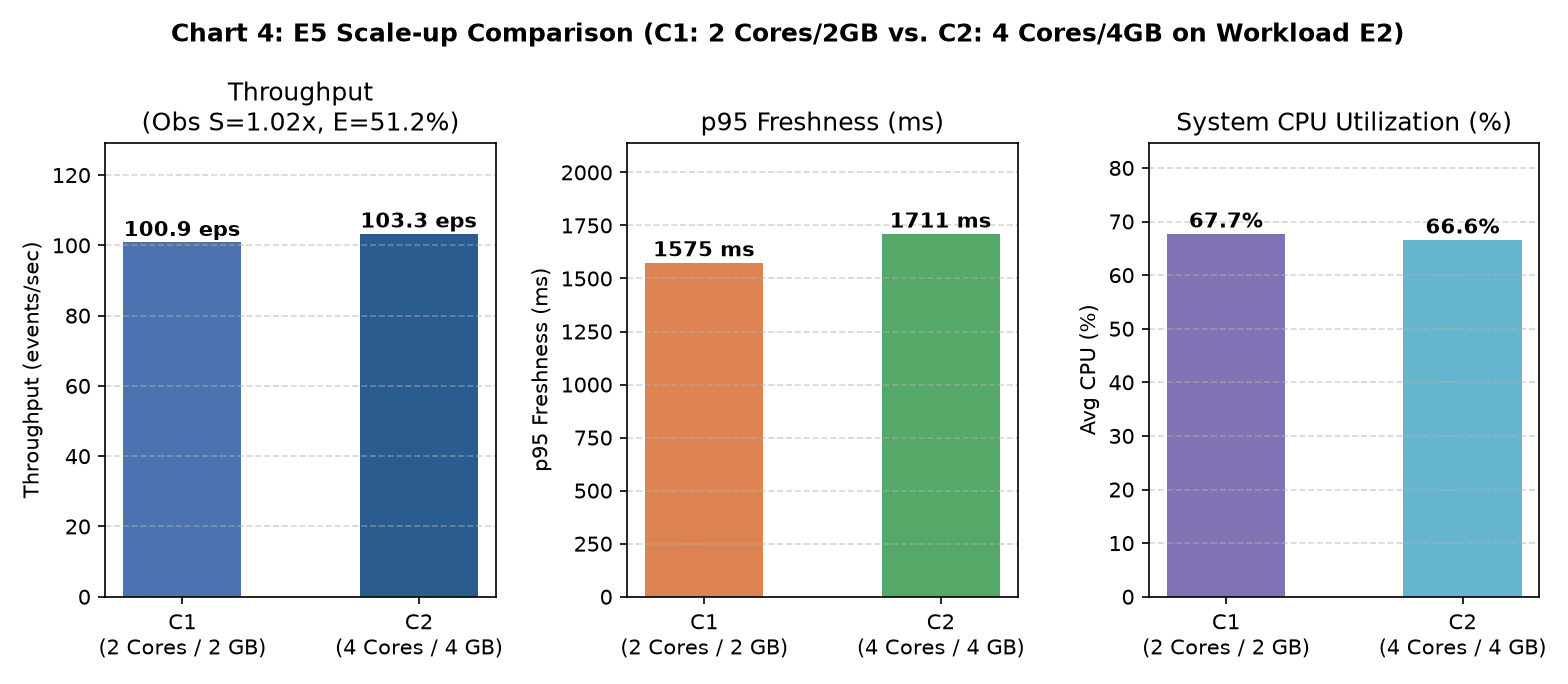
\includegraphics[width=0.68\textwidth]{../metrics/charts/chart4_e5_scaleup.png}
\caption{Chart~4: Vertical scale-up comparison (C1: 2 cores / 2\,GB vs.\ C2: 4 cores / 4\,GB on 100\,eps workload E2).}
\label{fig:c4}
\end{figure}

\textbf{Methodological Caveats.}
First, because C1 already keeps up with the 100\,eps producer (avg backlog 102.7), \emph{input rate caps throughput}; per evaluation rules, $S = 1.02\times$ and $E = 51.2\%$ are strictly \textbf{observed ratios under an input-rate cap}, not maximum cluster scaling capacity. Second, CPU cores and RAM were doubled simultaneously, so the \textbf{11.3\%} batch runtime reduction (15.45\,s $\rightarrow$ 13.71\,s) cannot be attributed purely to CPU. Third, three architectural ceilings prevent vertical Spark scaling from reducing speed-layer latency (p95: 1,575 $\rightarrow$ 1,711\,ms): Kafka has a single partition (limiting streaming consumers to 1), \texttt{collect()} pulls rows to one Python driver performing serial JDBC commits (\texttt{5.06\,ms/rec} in C2 vs.\ \texttt{4.99\,ms/rec} in C1), and host background load variance caused C1 to run slightly faster than the earlier \texttt{E2\_B} run on identical 2c/2g settings.

\section{Conclusions and Architectural Trade-offs}
\begin{enumerate}\setlength{\itemsep}{1pt}\setlength{\parskip}{0pt}
    \item \textbf{Does the system meet near-real-time requirements?} \textbf{Yes.} With E4 optimizations, Arch~B achieves \textbf{0.72\,s} median and \textbf{1.62\,s} p95 freshness at 100\,eps (vs.\ 38.9\,s / 68.8\,s in Batch-only) with zero count or sum error.
    \item \textbf{When is Lambda worthwhile, and at what cost?} Lambda pays off when sub-2-second freshness and exact batch recomputability are both mandatory. Its price is \textbf{+13--24\,pp} average CPU, \textbf{+0.3--0.7\,GB} RAM, higher serving query latency as unmerged speed rows accumulate, and dual-pipeline maintenance. When 30--60\,s staleness is tolerable, Batch-only is substantially cheaper and simpler.
    \item \textbf{Does scale-up scale proportionally with resources?} \textbf{No.} Doubling Spark cores and memory at 100\,eps trims batch duration by 11.3\% but delivers $S = 1.02\times$ ($E = 51.2\%$) due to input-rate capping, single-partition Kafka ingestion, and serial JDBC write bottlenecks.
    \item \textbf{Should the E4 optimization be applied?} \textbf{Yes.} Batched PostgreSQL upserts and tuned shuffle partitions outperform hardware scaling by nearly 3$\times$ on freshness at lower CPU and memory cost.
\end{enumerate}

\clearpage
\appendix
\section{Technical Verification: Serving Views and Live Reconciliation}

\textbf{PostgreSQL Serving Schema and Q1/Q2 Queries.}
All serving queries read views \texttt{v\_q1\_category} and \texttt{v\_q2\_total} defined in \texttt{sql/schema.sql}. Consistency is enforced by updating \texttt{batch\_views}, advancing \texttt{watermark\_meta.h\_seq}, and inserting \texttt{batch\_seen\_events} inside a single ACID transaction in \texttt{batch\_job.py}, while \texttt{speed\_job.py} deduplicates streaming writes via \texttt{PRIMARY KEY (event\_id)} and \texttt{ON CONFLICT (event\_id) DO NOTHING}.

\begin{table}[htbp]
\centering
\footnotesize
\begin{tabularx}{\textwidth}{|l|l|X|}
\hline
\rowcolor{headtint} \textbf{Object} & \textbf{Type} & \textbf{Purpose and Consistency Mechanism} \\
\hline
\texttt{watermark\_meta} & Table (1 row) & Stores authoritative batch high-water mark \texttt{h\_seq} ($H$) and \texttt{updated\_at}. \\
\rowcolor{rowtint} \texttt{batch\_views} & Table & Pre-aggregated \texttt{(category, cnt, sum\_cents, h\_seq)} for $\text{seq} \le H$; replaced atomically. \\
\texttt{speed\_events} & Table & Individual events ingested by Spark streaming; \texttt{PK(event\_id)}, indexed on \texttt{seq} and \texttt{(category, seq)}. \\
\rowcolor{rowtint} \texttt{batch\_seen\_events} & Table & Records earliest batch visibility timestamp per \texttt{event\_id} for Arch~A freshness tracking. \\
\texttt{v\_q1\_category} & View (Q1) & Unions \texttt{batch\_views} with \texttt{speed\_events WHERE seq > h\_seq} grouped by \texttt{category}. \\
\rowcolor{rowtint} \texttt{v\_q2\_total} & View (Q2) & Sums \texttt{v\_q1\_category} into global \texttt{system\_total\_count}, \texttt{system\_total\_sum\_cents}, and \texttt{current\_batch\_h}. \\
\hline
\end{tabularx}
\caption{PostgreSQL 15 serving schema objects (\texttt{sql/schema.sql} and instructor verification queries in \texttt{sql/queries.sql}).}
\end{table}

\textbf{Live Execution Proof and Automated Test Suite.}
Figure~\ref{fig:proof} is a live terminal screenshot captured with \texttt{hyprshot} (full log archived in \texttt{docs/verification\_proof.log}), confirming active localhost-bound Docker services (\texttt{lambda\_postgres}, \texttt{lambda\_kafka}), 8/8 passing unit tests in \texttt{tests/test\_pipeline.py} (covering contiguous watermark edge cases, raw-consumer Parquet filename contract, partial JSON tailing, active-window freshness sampling, SQL watermark deduplication, and error-preserving suite aggregation), live \texttt{v\_q2\_total} output (\texttt{12,001} events, \texttt{33,269,051} cents, $H=12001$), and 16/16 exact ground-truth reconciliation across the full benchmark matrix.

\begin{figure}[htbp]
\centering
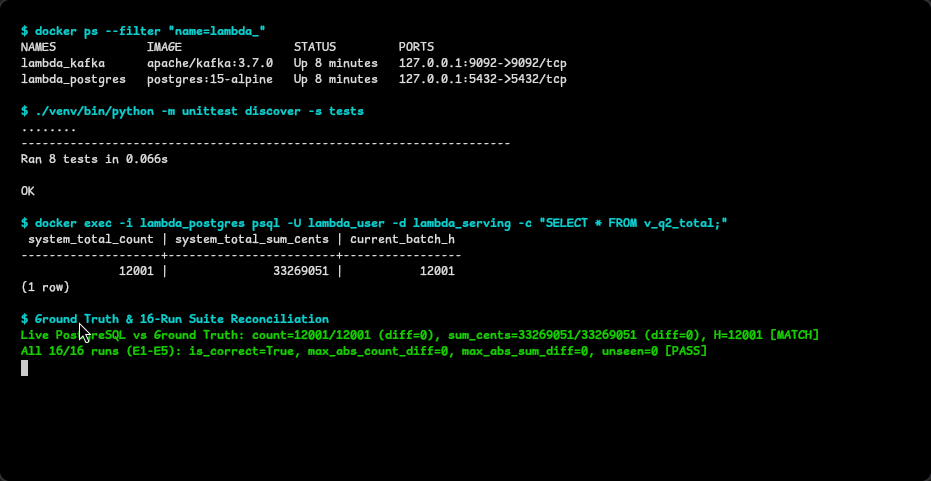
\includegraphics[width=0.95\textwidth]{../docs/verification_proof.png}
\caption{Live verification proof captured via \texttt{hyprshot}: Docker services, 8/8 unit tests, PostgreSQL Q2 query, and 16/16 run exactness.}
\label{fig:proof}
\end{figure}

\end{document}
